\section{Implementation}

\begin{frame}{Was ist eine Idee?}
	\begin{block}{Eigenschaften einer Idee}
		\begin{itemize}
			\item Qualität
			\item Komplexität
			\item "Weltanschauungswert"
			\item Komplexität abhängig von Qualität
		\end{itemize}
	\end{block}
\end{frame}

\begin{frame}[fragile]{Qualität}
	\begin{lstlisting}[language=C,basicstyle=\small,keywordstyle=\color{black}]
	 int chance = rand_int(1000, 0);
	  if(chance < BEST_IDEA_CHANCE){
	    i.a = rand_int(IDEA_MAX, 0);
	  }
	  else if(chance < MED_IDEA_CHANCE) {
	    i.a = rand_int((int) (IDEA_MAX * 0.66), 0);
	  }
	  else {
	    i.a = rand_int((int) (IDEA_MAX * 0.33), 0);
	  }
	  \end{lstlisting}
\end{frame}

\begin{frame}[fragile]{Komplexität}
	\begin{lstlisting}[language=C,basicstyle=\small,keywordstyle=\color{black}]
	int tempb = i.a + rand_int(2 * QUAL_CMPLXTY_DEP_RANGE + 1, - QUAL_CMPLXTY_DEP_RANGE);
	  if (0 <= tempb) {
	    if (tempb < IDEA_MAX) {
	      i.b = tempb;
	    } 
	    else i.b = IDEA_MAX - 1;
	  } 
	  else i.b = 0;
	\end{lstlisting}
\end{frame}

\begin{frame}[fragile] {Kommunikation \& Gewinner Berechnung}
	\begin{itemize}
	\item[1] Bewegen der Ideen (random)
	\item[2] Überprüfen ob Ideen miteinander in Wettkampf können 
	\end{itemize}
		\begin{lstlisting}[language=C,basicstyle=\small,keywordstyle=\color{black}]
			int convinceable = 1;
			if(abs((i1.c - i2.h)) > MAX_CWV_VS_HWV || abs((i2.c - i1.h)) > MAX_CWV_VS_HWV) {
	    		convinceable = 0;
	  		} 
	  		else if(complxdif > MAX_CMPLX_DIFF) {
	    		convinceable = 0;
		\end{lstlisting}	
	\begin{itemize}
	\item[3] Bestimmung der Winner-Idea 
	\item[4] Überschreiben der Loser-Idea
	\end{itemize}
\end{frame}

\begin{frame}[fragile]{Parallelisierungsschema}
	\begin{itemize}
		\item Implementierung des Felds durch 2D-Array von structs (Ideas)
		\item Es werden zwei Felder erstellt:
		\begin{lstlisting}[language=C,basicstyle=\small,keywordstyle=\color{black}]		
			malloc_idea_matrix(field)
			malloc_idea_matrix(field_new)
		\end{lstlisting}		
		\item sich bewegte Ideen werden in neues Feld kopiert
		\begin{lstlisting}
		#define copy_field_into_field_new()        
		    for_every(i, num_rows, {               
		        for_every(j, num_cols, {           
		            field_new[i][j] = field[i][j]; 
		          });                              
		    });
	    \end{lstlisting}		
	\end{itemize}	
\end{frame}

\begin{frame}{Parallelisierungsschema}
	\begin{picture}(0,0)
		\put(30,-80){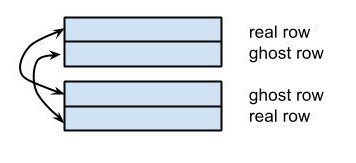
\includegraphics[scale=0.90]{finalPresentation/pics/real-ghost-rows.jpg}}
	\end{picture}
\end{frame}

\begin{frame}[fragile]{Parallelisierungsschema}
	\begin{itemize}
		\item horizontales Kommunikationsmuster
		\item am oberen bzw. unteren Rand ghost row
		\item Ziehen unabhängig von anderen Prozessen möglich
	\end{itemize}
\end{frame}

\begin{frame}{Parallelisierungsschema}
	\begin{picture}(0,230)
		\put(-120,0){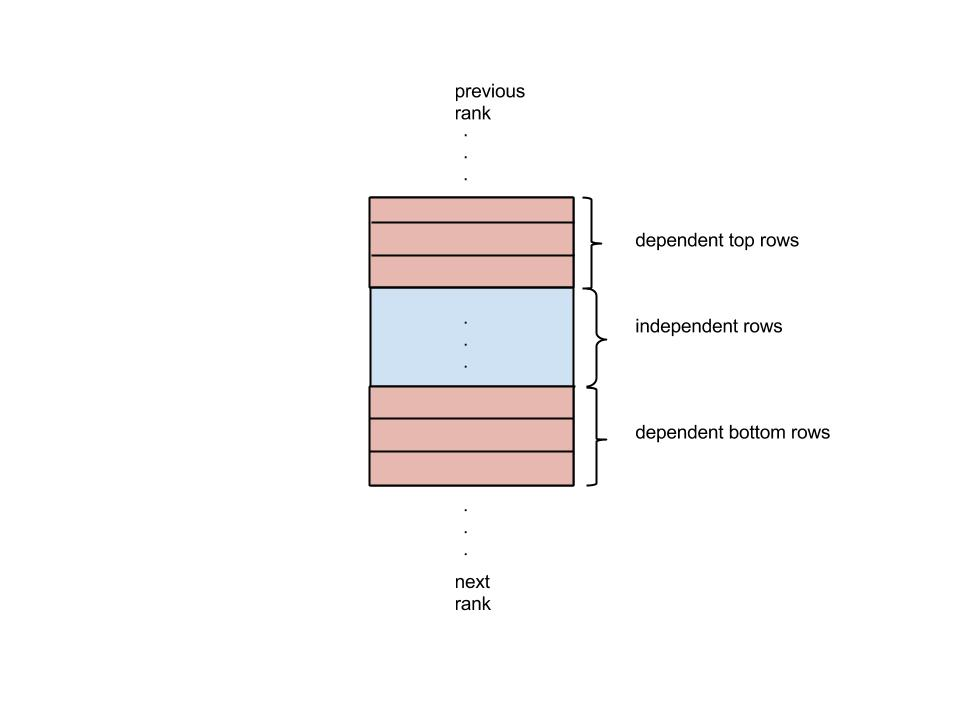
\includegraphics[height=8cm]{finalPresentation/pics/dependent-rows.jpg}}
		\put(170,180){\begin{minipage}[t]{0.4\linewidth}{
			\begin{itemize}
				\item[1.] Bewegung der independent ideas
				\item[2.] Bewegung der top dependent ideas, Kommunikation dieser
				\item[3.] Bewegung der bottom dependent ideas, Kommunikation dieser
			\end{itemize}
			}
		\end{minipage}}
	\end{picture}
\end{frame}

\begin{frame}[fragile]{Parallelisierungsschema}
\begin{lstlisting}[language=C,basicstyle=\small,keywordstyle=\color{black}]
#define send_ideas(ideas_arr, to, tag, req) 
  MPI_Isend(ideas_arr, num_cols, 
    mpi_idea_type, to, tag, MPI_COMM_WORLD, &req) 

#define receive_ideas_into(ideas_arr, from, tag, req) 
  MPI_Irecv(ideas_arr, num_cols, 
    mpi_idea_type, from, tag, MPI_COMM_WORLD, &req) 
\end{lstlisting}
\end{frame}

\begin{frame}[fragile]{Parallelisierungsschema}
\begin{lstlisting}[language=C,basicstyle=\small,breaklines=true,keywordstyle=\color{black}]
#define mpi_define_idea_type()                                               
  int blocklengths[5] = {1,1,1,1,1};                                  
  MPI_Datatype types[5] = {MPI_INT,MPI_INT,MPI_INT, MPI_INT, MPI_INT};       
  MPI_Datatype mpi_idea_type;                                                
  MPI_Aint offsets[5];                                                   
  offsets[0] = offsetof(Idea, a);                                            
  offsets[1] = offsetof(Idea, b);                                            
  offsets[2] = offsetof(Idea, c);                                            
  offsets[3] = offsetof(Idea, h);                                            
  offsets[4] = offsetof(Idea, empty);                                        
    MPI_Type_create_struct(5, blocklengths, offsets, types, &mpi_idea_type); 
    MPI_Type_commit(&mpi_idea_type);                                         
\end{lstlisting}
\end{frame}

\begin{frame}[fragile]{Visualisierung}
	\begin{itemize}
		\item lokale Visualisierung mithilfe von Pygame
		\item Pro Runde ein File
		\item im Nachhinein: Einlesen in Python
		\item Problem: Files werden zuerst auf dem Cluster gespeichert und muessen nach local kopiert werden
	\end{itemize}
\end{frame}

\begin{frame}{Optimierung}
	\begin{itemize}
		\item Ersetzen von Send/Recv mit Isend/Recv (10 \% Speedup)
	\end{itemize}
\end{frame}
